\documentclass[]{article}
\usepackage{lmodern}
\usepackage{amssymb,amsmath}
\usepackage{ifxetex,ifluatex}
\usepackage{fixltx2e} % provides \textsubscript
\ifnum 0\ifxetex 1\fi\ifluatex 1\fi=0 % if pdftex
  \usepackage[T1]{fontenc}
  \usepackage[utf8]{inputenc}
\else % if luatex or xelatex
  \ifxetex
    \usepackage{mathspec}
  \else
    \usepackage{fontspec}
  \fi
  \defaultfontfeatures{Ligatures=TeX,Scale=MatchLowercase}
\fi
% use upquote if available, for straight quotes in verbatim environments
\IfFileExists{upquote.sty}{\usepackage{upquote}}{}
% use microtype if available
\IfFileExists{microtype.sty}{%
\usepackage{microtype}
\UseMicrotypeSet[protrusion]{basicmath} % disable protrusion for tt fonts
}{}
\usepackage[margin=1in]{geometry}
\usepackage{hyperref}
\hypersetup{unicode=true,
            pdftitle={profiling hydrochemical dynamics in a rain-dominated water supply area: characterizing the Leech watershed using passive sampling techniques},
            pdfauthor={Hannah J McSorley},
            pdfborder={0 0 0},
            breaklinks=true}
\urlstyle{same}  % don't use monospace font for urls
\usepackage{longtable,booktabs}
\usepackage{graphicx,grffile}
\makeatletter
\def\maxwidth{\ifdim\Gin@nat@width>\linewidth\linewidth\else\Gin@nat@width\fi}
\def\maxheight{\ifdim\Gin@nat@height>\textheight\textheight\else\Gin@nat@height\fi}
\makeatother
% Scale images if necessary, so that they will not overflow the page
% margins by default, and it is still possible to overwrite the defaults
% using explicit options in \includegraphics[width, height, ...]{}
\setkeys{Gin}{width=\maxwidth,height=\maxheight,keepaspectratio}
\IfFileExists{parskip.sty}{%
\usepackage{parskip}
}{% else
\setlength{\parindent}{0pt}
\setlength{\parskip}{6pt plus 2pt minus 1pt}
}
\setlength{\emergencystretch}{3em}  % prevent overfull lines
\providecommand{\tightlist}{%
  \setlength{\itemsep}{0pt}\setlength{\parskip}{0pt}}
\setcounter{secnumdepth}{0}
% Redefines (sub)paragraphs to behave more like sections
\ifx\paragraph\undefined\else
\let\oldparagraph\paragraph
\renewcommand{\paragraph}[1]{\oldparagraph{#1}\mbox{}}
\fi
\ifx\subparagraph\undefined\else
\let\oldsubparagraph\subparagraph
\renewcommand{\subparagraph}[1]{\oldsubparagraph{#1}\mbox{}}
\fi

%%% Use protect on footnotes to avoid problems with footnotes in titles
\let\rmarkdownfootnote\footnote%
\def\footnote{\protect\rmarkdownfootnote}

%%% Change title format to be more compact
\usepackage{titling}

% Create subtitle command for use in maketitle
\providecommand{\subtitle}[1]{
  \posttitle{
    \begin{center}\large#1\end{center}
    }
}

\setlength{\droptitle}{-2em}

  \title{profiling hydrochemical dynamics in a rain-dominated water supply area:
characterizing the Leech watershed using passive sampling techniques}
    \pretitle{\vspace{\droptitle}\centering\huge}
  \posttitle{\par}
  \subtitle{DRAFT -- NSERC forWater Pacific Maritime Masters Thesis Project}
  \author{Hannah J McSorley}
    \preauthor{\centering\large\emph}
  \postauthor{\par}
      \predate{\centering\large\emph}
  \postdate{\par}
    \date{2019-11-11}


\begin{document}
\maketitle

\subsection{Acronyms}\label{acronyms}

\begin{longtable}[]{@{}lll@{}}
\toprule
\begin{minipage}[b]{0.11\columnwidth}\raggedright\strut
Acronym\strut
\end{minipage} & \begin{minipage}[b]{0.09\columnwidth}\raggedright\strut
Term\strut
\end{minipage} & \begin{minipage}[b]{0.16\columnwidth}\raggedright\strut
Definition\strut
\end{minipage}\tabularnewline
\midrule
\endhead
\begin{minipage}[t]{0.11\columnwidth}\raggedright\strut
NOM\strut
\end{minipage} & \begin{minipage}[t]{0.09\columnwidth}\raggedright\strut
natural organic matter\strut
\end{minipage} & \begin{minipage}[t]{0.16\columnwidth}\raggedright\strut
diverse carbon-based compounds found in natural, engineered, terrestrial
and aquatic environments\strut
\end{minipage}\tabularnewline
\begin{minipage}[t]{0.11\columnwidth}\raggedright\strut
DOM\strut
\end{minipage} & \begin{minipage}[t]{0.09\columnwidth}\raggedright\strut
dissolved organic matter\strut
\end{minipage} & \begin{minipage}[t]{0.16\columnwidth}\raggedright\strut
organic compounds operationally defined as finer than 0.45 um in
diameter\strut
\end{minipage}\tabularnewline
\begin{minipage}[t]{0.11\columnwidth}\raggedright\strut
DOC\strut
\end{minipage} & \begin{minipage}[t]{0.09\columnwidth}\raggedright\strut
dissolved organic carbon\strut
\end{minipage} & \begin{minipage}[t]{0.16\columnwidth}\raggedright\strut
organic carbon compounds operationally defined as finer than 0.45 um in
diameter. The majority of DOM is DOC.\strut
\end{minipage}\tabularnewline
\begin{minipage}[t]{0.11\columnwidth}\raggedright\strut
NPOC\strut
\end{minipage} & \begin{minipage}[t]{0.09\columnwidth}\raggedright\strut
non-purgeable organic carbon\strut
\end{minipage} & \begin{minipage}[t]{0.16\columnwidth}\raggedright\strut
instrumental parameter measured to quantify organic carbon (e.g.~on a
Shimadzu TOC-V analyzer). An aqueous sample is acidified to below pH 2
to convert inorganic carbon (e.g.~carbonates) to carbon dioxide (CO2),
the sample is then sparged with hydrocarbon-free air to drive off CO2,
then the sample is combusted at high temperatures to convert the
remaining organic carbon to CO2 which is detected with a non-dispersive
infrared gas analyzer.\strut
\end{minipage}\tabularnewline
\begin{minipage}[t]{0.11\columnwidth}\raggedright\strut
DBP-FP\strut
\end{minipage} & \begin{minipage}[t]{0.09\columnwidth}\raggedright\strut
Disinfection By-Product Formation Potential\strut
\end{minipage} & \begin{minipage}[t]{0.16\columnwidth}\raggedright\strut
The likelihood of creating DBPs(e.g.~trihalomethanes, halogenic acetic
acids, Haloacetonitrils, haloketons) when natural source water is
chlorinated\strut
\end{minipage}\tabularnewline
\begin{minipage}[t]{0.11\columnwidth}\raggedright\strut
LWSA\strut
\end{minipage} & \begin{minipage}[t]{0.09\columnwidth}\raggedright\strut
Leech Water Supply Area\strut
\end{minipage} & \begin{minipage}[t]{0.16\columnwidth}\raggedright\strut
Future water supply area anticipated to supplement the primary water
supply (Sooke Reservoir) for the Greater Victoria Area via inter-basin
transfer. LWSA is the research site for this thesis' field work.\strut
\end{minipage}\tabularnewline
\begin{minipage}[t]{0.11\columnwidth}\raggedright\strut
CRD\strut
\end{minipage} & \begin{minipage}[t]{0.09\columnwidth}\raggedright\strut
Capital Regional District\strut
\end{minipage} & \begin{minipage}[t]{0.16\columnwidth}\raggedright\strut
The governing/municipal body for the Greater Victoria Area, and the
managing group for water supply and watershed management. The CRD are
partners in the forWater Network and hosted this thesis research in the
Leech Water Supply Area.\strut
\end{minipage}\tabularnewline
\begin{minipage}[t]{0.11\columnwidth}\raggedright\strut
GVWSA\strut
\end{minipage} & \begin{minipage}[t]{0.09\columnwidth}\raggedright\strut
Greater Victoria Water Supply Area\strut
\end{minipage} & \begin{minipage}[t]{0.16\columnwidth}\raggedright\strut
20,549 hectares of protected drinking water catchment lands owned and
operated by the Capital Regional District. Includes the Sooke Lake
watershed and reservoir (primary supply source), Goldstream watershed
and reservoir system (secondary supply) and the Leech River watershed
(future water supply area, and the study site of this thesis
research)\strut
\end{minipage}\tabularnewline
\bottomrule
\end{longtable}

\subsection{Acknowledgements}\label{acknowledgements}

This research work would not have been possible without the support and
accommodation of the Capital Regional District (CRD) Watershed
Protection and Management Division, Integrated Water Services (IWS),
Victoria, BC. In particular, Hannah McSorley would like to acknowledge
the help, support and assistance provided by:

\begin{itemize}
\tightlist
\item
  Tobi Gardner \textbar{} Senior Hydrologist
\item
  Joel Ussery \textbar{} Manager, Resource Planning
\item
  Annette Constabel \textbar{} Senior Manager
\item
  Christoph Moch \textbar{} Manager, Water Quality Operations
\item
  Kathy Haesevoats \textbar{} Watershed Technologist
\item
  Ryan Biggs \textbar{} Watershed Technician 2, Resource Planning(?)
\item
  Burn Hemus \textbar{} ?
\item
  Jessica Dupuis \textbar{} ?? Water Quality Operations
\item
  Nigel Burrows \textbar{} Manager Watershed Fire, Security and
  Emergency Response
\item
  Patrick McCoubrey \textbar{} Security Chargehand
\item
  Devon Barnes, RPF, MSc \textbar{} Watershed Protection Senior
  Supervisor
\end{itemize}

This research also would not have been possible without the academic
support and encouragement from academic supervisors and partners with
the NSERC forWater Network for Forested Drinking Water Source Protection
Technologies:

\begin{itemize}
\tightlist
\item
  Bill Floyd \textbar{} Academic co-supervisor \textbar{} Adjunct
  Professor, Geography, Vancouver Island University \& Research
  Hydrologist, BC-FLNRO
\item
  Mark Johnson \textbar{} Academic co-supervisor \textbar{} Professor
  and Canada Research Chair, University of British Columbia
\item
  Mike Stone \textbar{} Professor, Faculty of Environment, Dept. of
  Geography and Environmental Management, University of Waterloo
\item
  Dana Harriman \textbar{} Network Manager, University of Waterloo
\item
  Monica Emelko \textbar{} Principle Investigator, Scientific Director,
  University of Waterloo
\item
  Uldis Silins \textbar{} Co-Principle Investigator, Co-Scientific
  Director, University of Alberta
\item
  Danielle Lindamood \textbar{}(former) Knowledge Mobilization Manager
\item
  Allie Dusome \textbar{} Communications Officer, the Water Institute,
  University of Waterloo
\item
  Axel Anderson \textbar{} Professor, Faculty of Agricultural, Life and
  Environmental Science, Renewable Resources Dept., University of
  Alberta
\end{itemize}

\section{Introduction}\label{introduction}

\subsection{Source water quality and rain
events}\label{source-water-quality-and-rain-events}

\subsubsection{Stormflow and sampling (including passive sampling
techniques and
advantages)}\label{stormflow-and-sampling-including-passive-sampling-techniques-and-advantages}

\subsubsection{Disscolved organic carbon and water
treatment}\label{disscolved-organic-carbon-and-water-treatment}

\subsubsection{Dissolved organic carbon and other
parameters}\label{dissolved-organic-carbon-and-other-parameters}

\subsection{Greater Victoria Regional Water Supply
System}\label{greater-victoria-regional-water-supply-system}

The Capital Regional District (CRD) owns and operates the water supply
system for the Greater Victoria region. As a water purveyor, CRD
supplies an average of 130 million liters of treated water to customers
each day (Capital Region District 2017). The provision of safe and
sustainable drinking water is regulated by three bodies above the CRD:
federal, provincial, and regional. Health Canada (federal government)
publishes Canadian Drinking Water Quality Guidelines which outline
quantitative bounds for microbial, chemical, radiological parameters and
physical aesthetic characteristics of safe drinking water. Through the
Public Health Act and Regulation, the Drinking Water Protection Act and
the Water Sustainability Act, the province of British Columbia sets
requirements for planning, reporting and regualting of drinking water
providers. The Vancouver Island Health Authority, Island Health, is the
agency that the CRD reports to regarding water quality information and
provincial legislation.

The Greater Victoria Water Supply Area (GVWSA) includes 20,549 hectares
(205.49 km\textsuperscript{2}) of protected drinking water catchment
lands. The primary water supply is sourced from Sooke reservoir,
secondary supply source is Goldstream reservoir and the designated
(supplemental) future water supply is the Leech River watershed.
Unfiltered source water is first treated with ultraviolet light (to
deactivate parasites) and free chlorine (to deactive bacteria and
viruses); secondarily, ammonia is added to produce chloramine, a
long-lasting disinfectant (Capital Region District 2017).

The Leech River watershed is adjacent to Sooke Reservoir, which is the
primary water supply for the Greater Victoria Area. In anticipation of
future water demands and uncertainty related to rainfall and climate
change, the Capital Regional District (CRD) purchased 9,628 hectares
(about 92\%) of the Leech River watershed in 2007 () and 2010 (), and
designated the Leech Water Supply Area (LWSA) as future supplemental
water supply. The Leech Tunnel was constructed in the 1980's to transfer
Leech River water into the Sooke watershed. The Tunnel is not currently
operational, and it's anticipated that inter-basin transfer won't be
required until 2050 or later.

\begin{quote}
To prepare for the eventual use of the LWSA, further work is required to
plan for the water quality impacts of the different raw water sources,
rehabilitation of the water supply area forests and drainage structures,
and infrastructure necessary to convey the LWSA flows into Sooke Lake
Reservoir \textasciitilde{}(Capital Region District 2017)
\end{quote}

\section{Research area: Leech River
Watershed}\label{research-area-leech-river-watershed}

The Leech River watershed is located on south-east Vancouver Island,
British Columbia, Canada. The area is in the Coastal Western Hemlock
Biogeoclimatic Zone. The hydroclimatic regime for the Leech watershed is
pluvial (rain-dominated climate). Annual rainfall is typically between
xxxx - yyyy mm (\textasciitilde{}2500 mm/yr). This areas has a strong
seasonal distribution of rainfall: approximately 90\% of rain falls from
September to April, with only about 10\% of annual rainfall occurring
from May to August. The watershed forests are dominated by western red
cedar, hemlock, and Douglas fir.

Prior to purchase by the CRD, the LWSA was privately managed forest
land. Approximately 96\% of the Leech watershed was harvested by clear
cut. The majority \textbf{(?\% of total area)} of the LWSA forests are
under 30 years of age. Now designated as a Water Supply Area, the Leech
is managed by the CRD for source water protection, ecosystem services,
and forest resilience. As forest fires pose a serious threat to
monocultured and even-aged stands (\textbf{REFS}), particularly during
the drought of summer, forest fuel management is a key preemptive risk
reduction for the CRD. *** DID LEECH GET P.C.T \& WAS IT PLANTED** --
\{** pre-commercial thinning 5-10yrs after regen, versus 20 yrs, versus
problem**\}

The Leech River system is composed of three main stem rivers, numerous
tributaries, and four small headwater lakes. The rivers are flashy: they
respond rapidly to rain events, rising and falling dramatically. The
hydrology of the LWSA is poorly understood, as is the water quality. In
the mid-1980's, some water was transfered from the Leech River into
Deception Gulch and Reservoir (adjacent but physically separated from
Sooke Reservoir). The mixing resulted in biological water quality
problems that included odour and raised concerns about the operational
usage of the existing tunnel. The Leech River Tunnel and anticipated
inter-basin transfer will provide interesting research opportunities,
but is beyond the scope of this thesis research. Before work is done on
inter-basin transfers, the hydrology and water quality of the Leech
River system need to be better understood. The timing and magnitude of
flows is important to accommodate the water license that the CRD holds
for \textbf{winter} withdraws from the Leech. Understanding source water
quality is an essential part of managing water supply and a foundation
of the multiple barrier approach to clean drinking water.

This thesis research bridges the CRD's commitment to planning for the
future use of the LWSA with the objectives of the forWater Network, by
establishing an understanding of ``natural'' hydrochemical variability
across a forested source water area. The caveat on the term ``natural''
is to say that the majority (** HOW MANY \textbf{) of forested
ecosystems on Vancouver Island are second growth forests which have been
previously been harvested. The forest industry is a crucial component of
BC's economic system, and essential to the lives that people on the
coast are accustomed to. (} facts about forestry in BC **).

\subsection{Research Objectives}\label{research-objectives}

As part of the Pacific Maritime Reserch Platform in forWater's
\emph{`Watershed Science and Forest Management'} Theme, this thesis
research was carried out in partnership with the CRD in the future water
supply area of the Leech River watershed. This research project was
designed to contribute to the characterization of the LWSA and better
our understanding of spatial and temporal variability in DOC dynamics
across a second growth forested catchment. This work set out to
establish a baseline understanding of hydrologic responses and water
quality variabilty in rivers across the LWSA, contributing to the CRDs
ongoing pursuit of characterizing the Leech. This thesis research
approach included advanced synoptic sampling within stormflow,
supplemented with standard grab samples between storm events and during
summer baseflow. Discrete samples of river water were collected
passively during the rising limb of stormflow xx(falling limb prototype
in progress)xx using low-powered, low-cost, custom-built vertical rack
samplers including water level loggers and reference staff gauges. By
collecting samples during stormflow, rather than only opportunitic grab
sampling, a more robust understanding of water quality dynamics was
achieved. Using low-powered passive sampling techniques allowed for six
(6) research sites to be equipped with monitoring/sampling racks,
providing fairly good spatial resolution of hydrochemical variability
across the watershed.

The research presented in this thesis focuses on describing the spacial
and temporal patterns and trends in water quality across the Leech River
watershed, an area with a history of extensive forest harvest. Spatial
variability was addressed by setting up parallel monitoring stations at
six locations respresenting the headwaters and three main stem rivers of
the Leech River system. Temporal variability was addressed at the
seasonal scale via continuous 16 month study (October 2018 to February
2020), and on a shorter timeframe, at the scale of stormflow. The
research questions and hypotheses addressed here were:

\begin{enumerate}
\def\labelenumi{\arabic{enumi}.}
\tightlist
\item
  How do water quality and hydrologic response vary across the Leech
  Water Supply Area?
\end{enumerate}

\begin{itemize}
\tightlist
\item
  Hypothesis 1.1: The headwater site with wetland characteristics will
  have the highest DOC concentration.
\item
  Hypothesis 1.2: DOC concentrations will decrease from headwaters to
  mouth due to dilution effects from the increasing drainage area.
\end{itemize}

\begin{enumerate}
\def\labelenumi{\arabic{enumi}.}
\setcounter{enumi}{1}
\tightlist
\item
  What are the temporal patterns in water quality changes, both
  seasonally and within stormflow?

  \begin{itemize}
  \tightlist
  \item
    Hypothsis 2.1: Compared to late wet-season rain events, early
    wet-season storms will yield the highest concentrations of stream
    DOC due to flushing of terestrial organic matter.
  \item
    Hypothesis 2.2: Baseflow DOC concentrations will increase over the
    summer due to concentration of instream organic matters.
  \end{itemize}
\item
  What are the patterns in hydrochemical dynamics at the future point of
  diversion (Leech Tunnel), and what are the treatment implications?

  \begin{itemize}
  \tightlist
  \item
    Hypothesis 3.1: The Tunnel site will integrate characteristics of
    each of the nested catchments (sites 1-5) with a slightly stronger
    signature of the West Leech River due to close proximity of it's
    confluence.
  \item
    Hypotheiss 3.2: The DOC concentration at the Tunnel site will be the
    lowest of all six sites and will not exceed drinking water quality
    guidelines.
  \end{itemize}
\end{enumerate}

Research objectives, based on these questions, were to:

\begin{itemize}
\tightlist
\item
  Monitor water quality and water level across the LWSA,\\
\item
  Identify differences and similarities between sites (spatial) and
  variations over time (temporal, short and relatively long scales),
\item
  Collaborate with forWater Network partners to assess the implications
  for drinking water treatment and relate findings to sub-basin
  characteristics.
\end{itemize}

Tasks related to these research objectives were: site selection, method
development, field installations, sample collection and analysis, data
analysis and interpretation

\begin{figure}
\centering
\includegraphics{images/MSc_tasksflowchart.jpg}
\caption{Masters thesis task flowchart}
\end{figure}

\subsection{Research sites}\label{research-sites}

Six sites were selected across the Leech Water Supply Area. The six
research sites represent five nested catchments and the entire water
supply area basin defined from the point of (future) diversion, the
Leech Tunnel.

\begin{longtable}[]{@{}lllrr@{}}
\toprule
Site Number & Site Name & Characteristic & Drainage Area
(km\textsuperscript{2}) & Elevation (m a.s.l)\tabularnewline
\midrule
\endhead
1 & Weeks Outlet & Wetland-draining headwaters & 16.1 &
XX\tabularnewline
2 & Chris Creek & Headwaters & 9.6 & XX\tabularnewline
3 & Leech Head & Mainstem river head & 26.2 & XX\tabularnewline
4 & Cragg Creek & Mainstem river & 37.1 & XX\tabularnewline
5 & West Leech & Mainstem river & 35.2 & XX\tabularnewline
6 & Leech Tunnel & Future diversion point & 98.7 & XX\tabularnewline
\bottomrule
\end{longtable}

\_*Sites 1 and 2 monitor subcatchments of the site 3 drainage area.\_

Note that Strahler order was used to define stream orders, such that a
headwater creek is assigned first order, and the confluence of two
headwater streams creates a second order stream, two second order
streams join to become a third order, and so on (i.e headwaters are
lowest number, mouth is highest).

\paragraph{1. Weeks Outlet}\label{weeks-outlet}

Jordan Meadows wetland is located in the northwest of Leech River
watershed, it drains to the east and joins the outflow of Weeks Lake
(south end of the lake). The wetland and lake outflow streams join and
flow east to Research Site \#1, ``Weeks Outlet'', which is a third order
stream (Strahler) of the western headwaters of Leech River. This
research site has a drainage area of approximately 16
km\textsuperscript{2}. The channel is fairly straight and bed material
is primarily silt/clay. The water at this site was noteabley
tannin-coloured. This research site was located about 0.4 km west
(upstream) of the confluence with Chris Creek.

A large culvert upstream of the monitoring site was replace with a
bridge in August of 2019. The culvert had been perched above the
streambed level and was obstructing the movement of fish and water flow.
Prior to the culvert removal, several groundwater seeps were observed
downstream; these seeps maintained base flow of summer waters in this
low-relief stream reach. There were high levels of iron (above guidlines
for aesthetic objectives) in the water downstream of the culvert,
possibly due to culvert rust.

\begin{verbatim}
![](images/XXXXX.jpg){width=50%} ![](images/YYYY.jpg){width=50%}
\end{verbatim}

\paragraph{2. Chris Creek}\label{chris-creek}

Chris Creek is the western headwaters of Leech River. This research site
is approximately 0.2 km east (upstream) of the confluence with the Weeks
Outlet stream. The study site on Chris Creek monitors waters draining
from approximately 9.6 km\textsuperscript{2} of forested land, including
a small lake (Worley Lake). The monitoring site of Chris Creek was
downstream of a bridge, on a slightly sinuous reach with boulders and
bedrock dominated morphology and turbulent cascading step-pools. There
is a brige that passes over Chris Creek and a large collection of coarse
woody debris downstream of the bridge, upstream of the monitoring site.

\begin{verbatim}
![](images/XXXXX.jpg){width=50%} ![](images/YYYY.jpg){width=50%}
\end{verbatim}

\paragraph{3. Leech Head}\label{leech-head}

Research site 3 was approxiamtely 1.4 km downstream of the confluence of
Weeks Outlet stream and Chris Creek. The ``Leech Head'' study site was
in a deep pool between riffles, it's a 4th order stream with
predominantly Schist bedrock and fairly low relief
(\textasciitilde{}2\%) and relatively straight morphology. The water at
this site was often coloured by tannins (likely from the Weeks outlet
stream contributions). There once was a logging bridge across the river
at this site, and some rip-rap remains on either bank.

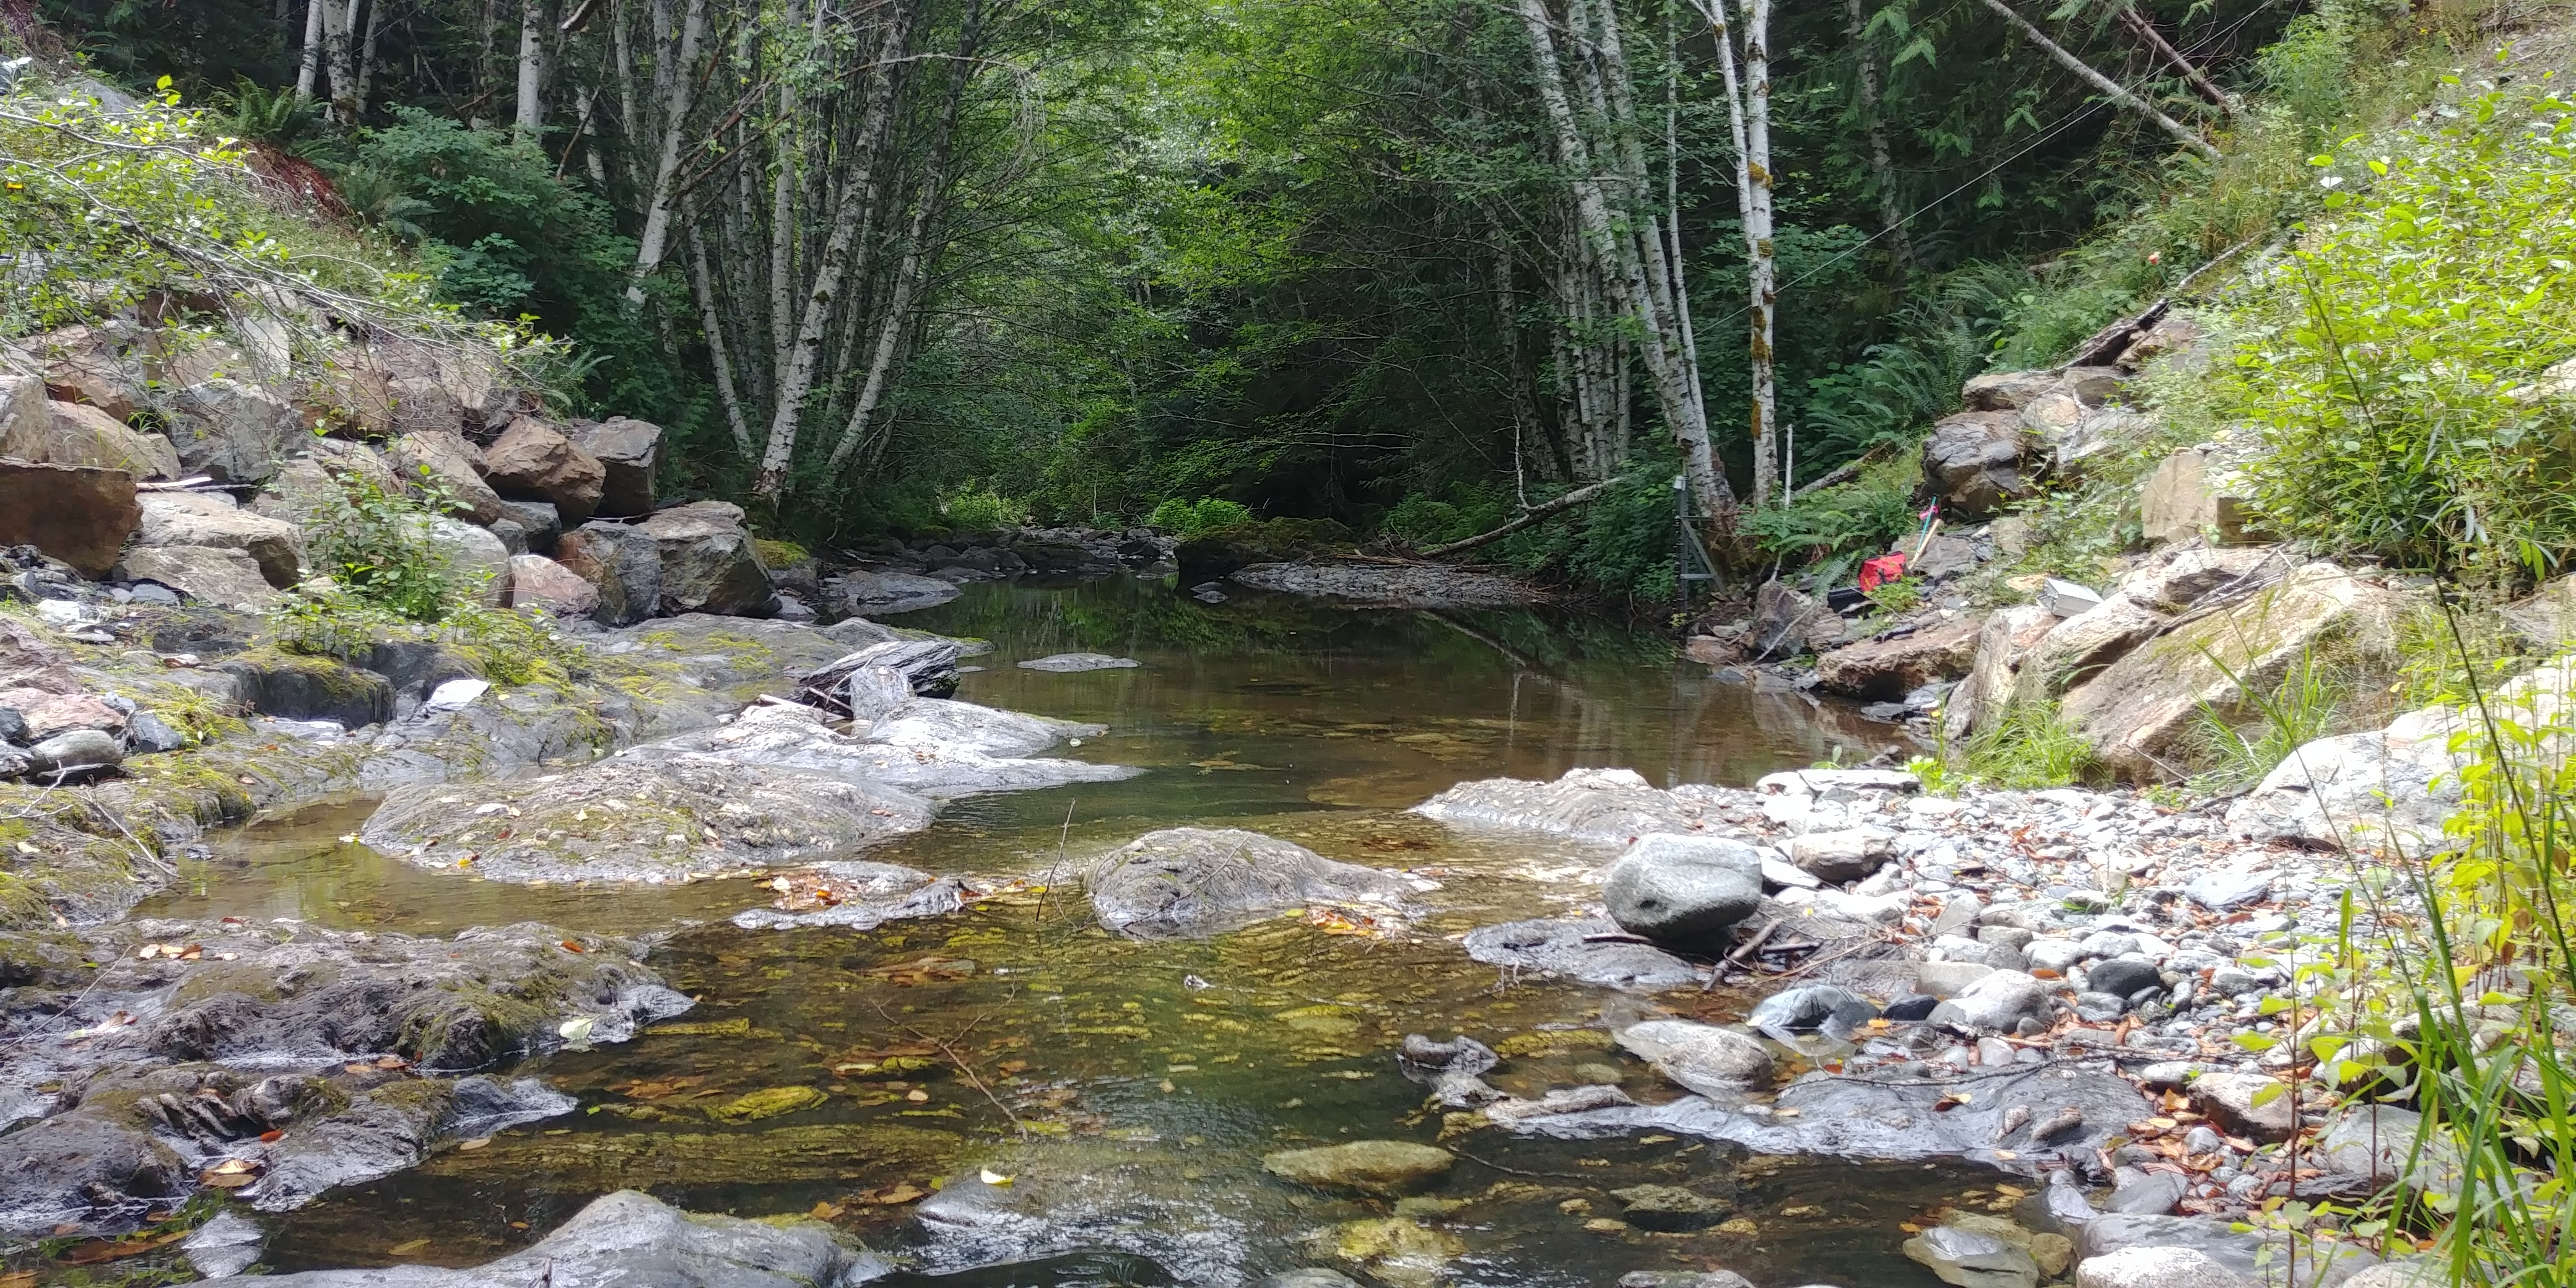
\includegraphics[width=0.25000\textwidth]{images/LeechHead_lowflow_201908.jpg}
\includegraphics{images/MMMM.jpg}

\paragraph{4. Cragg Creek}\label{cragg-creek}

Cragg Creek is a mainstem river that originates in the east of the Leech
River watershed. Cragg Creek is a 4th order stream and this research
site location has a drainage area of approximately 37
km\textsuperscript{2}. The Cragg Creek research station was installed
upstream of a road bridge, at a CRD hydrological monitoring site
(installed over the span of this thesis project). The bed morphology at
this site is Schist bedrock and the stream is straight channel with
fairly high width-to-depth ratio. Upstream of the bridge Cragg Creek
flows turbulently along a low slope, and downstream of the bridge it
cascades into several deep pools. From the Cragg Creek research site,
the river flows approximately 4.5 km through a steep revine to
confluence with the Leech River (this confluence is around 6 km
downstream of the Leech Head site, site \#3).

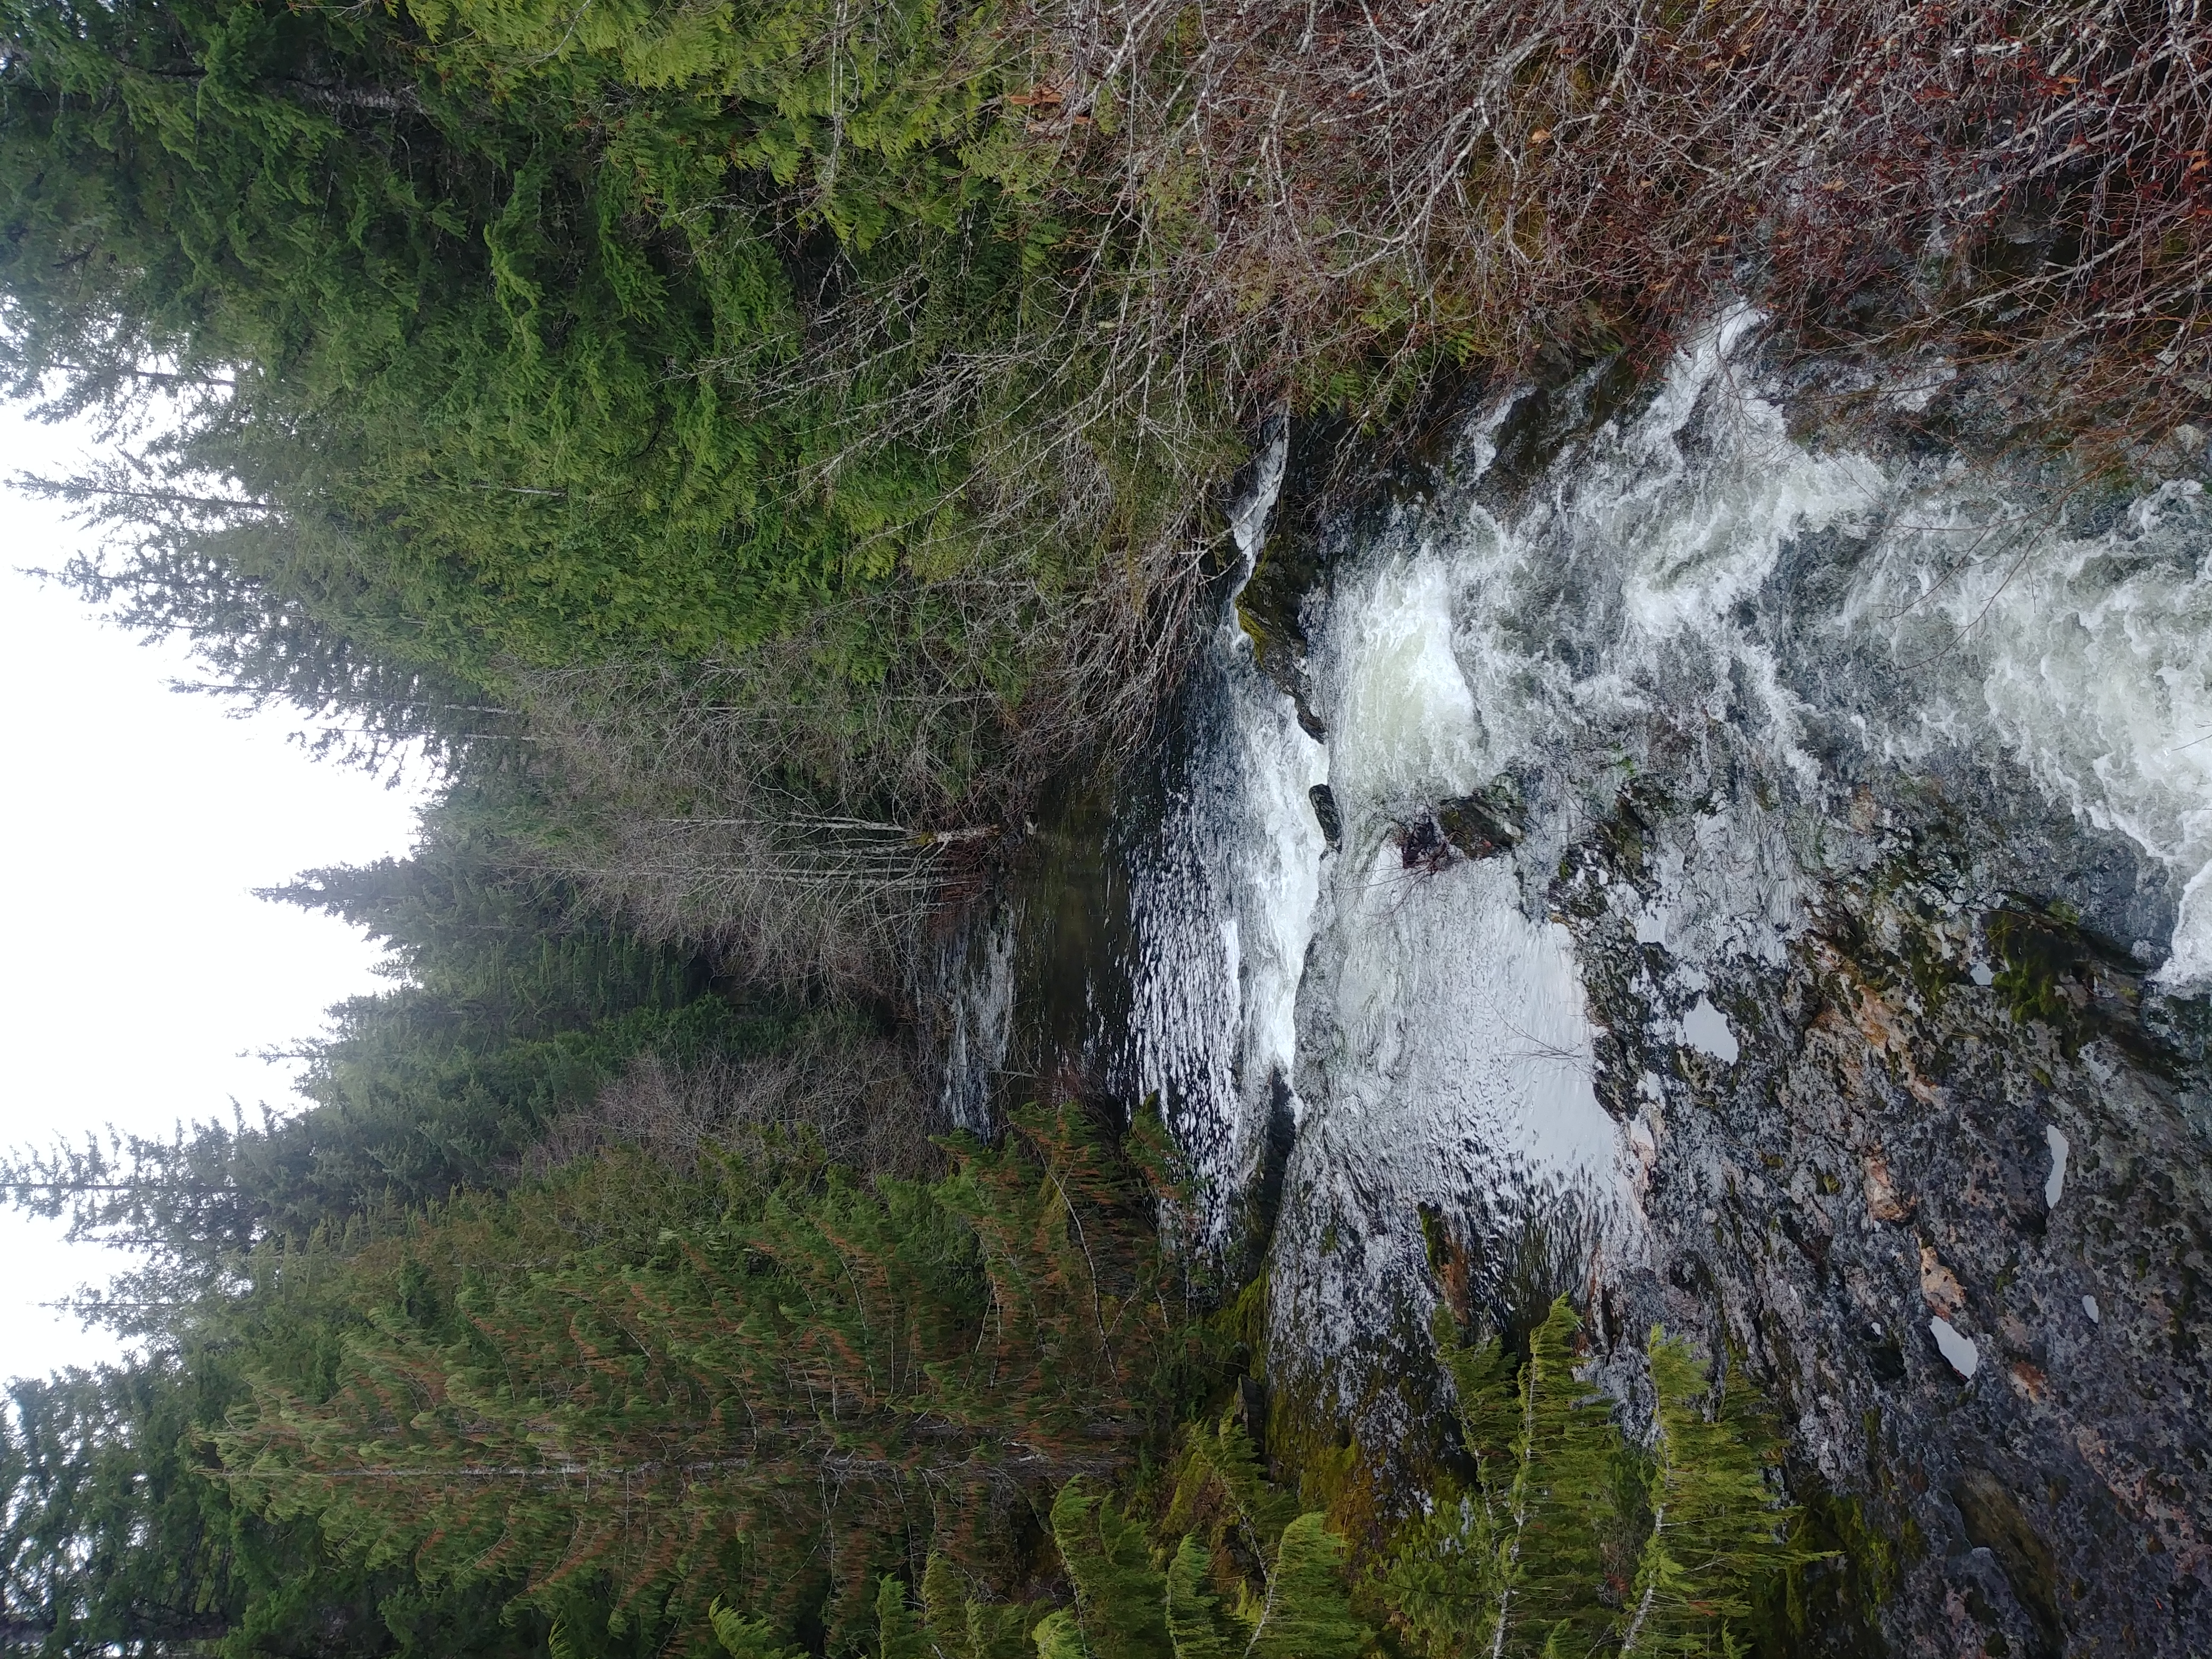
\includegraphics{images/Cragg_downstream_20190410.jpg}
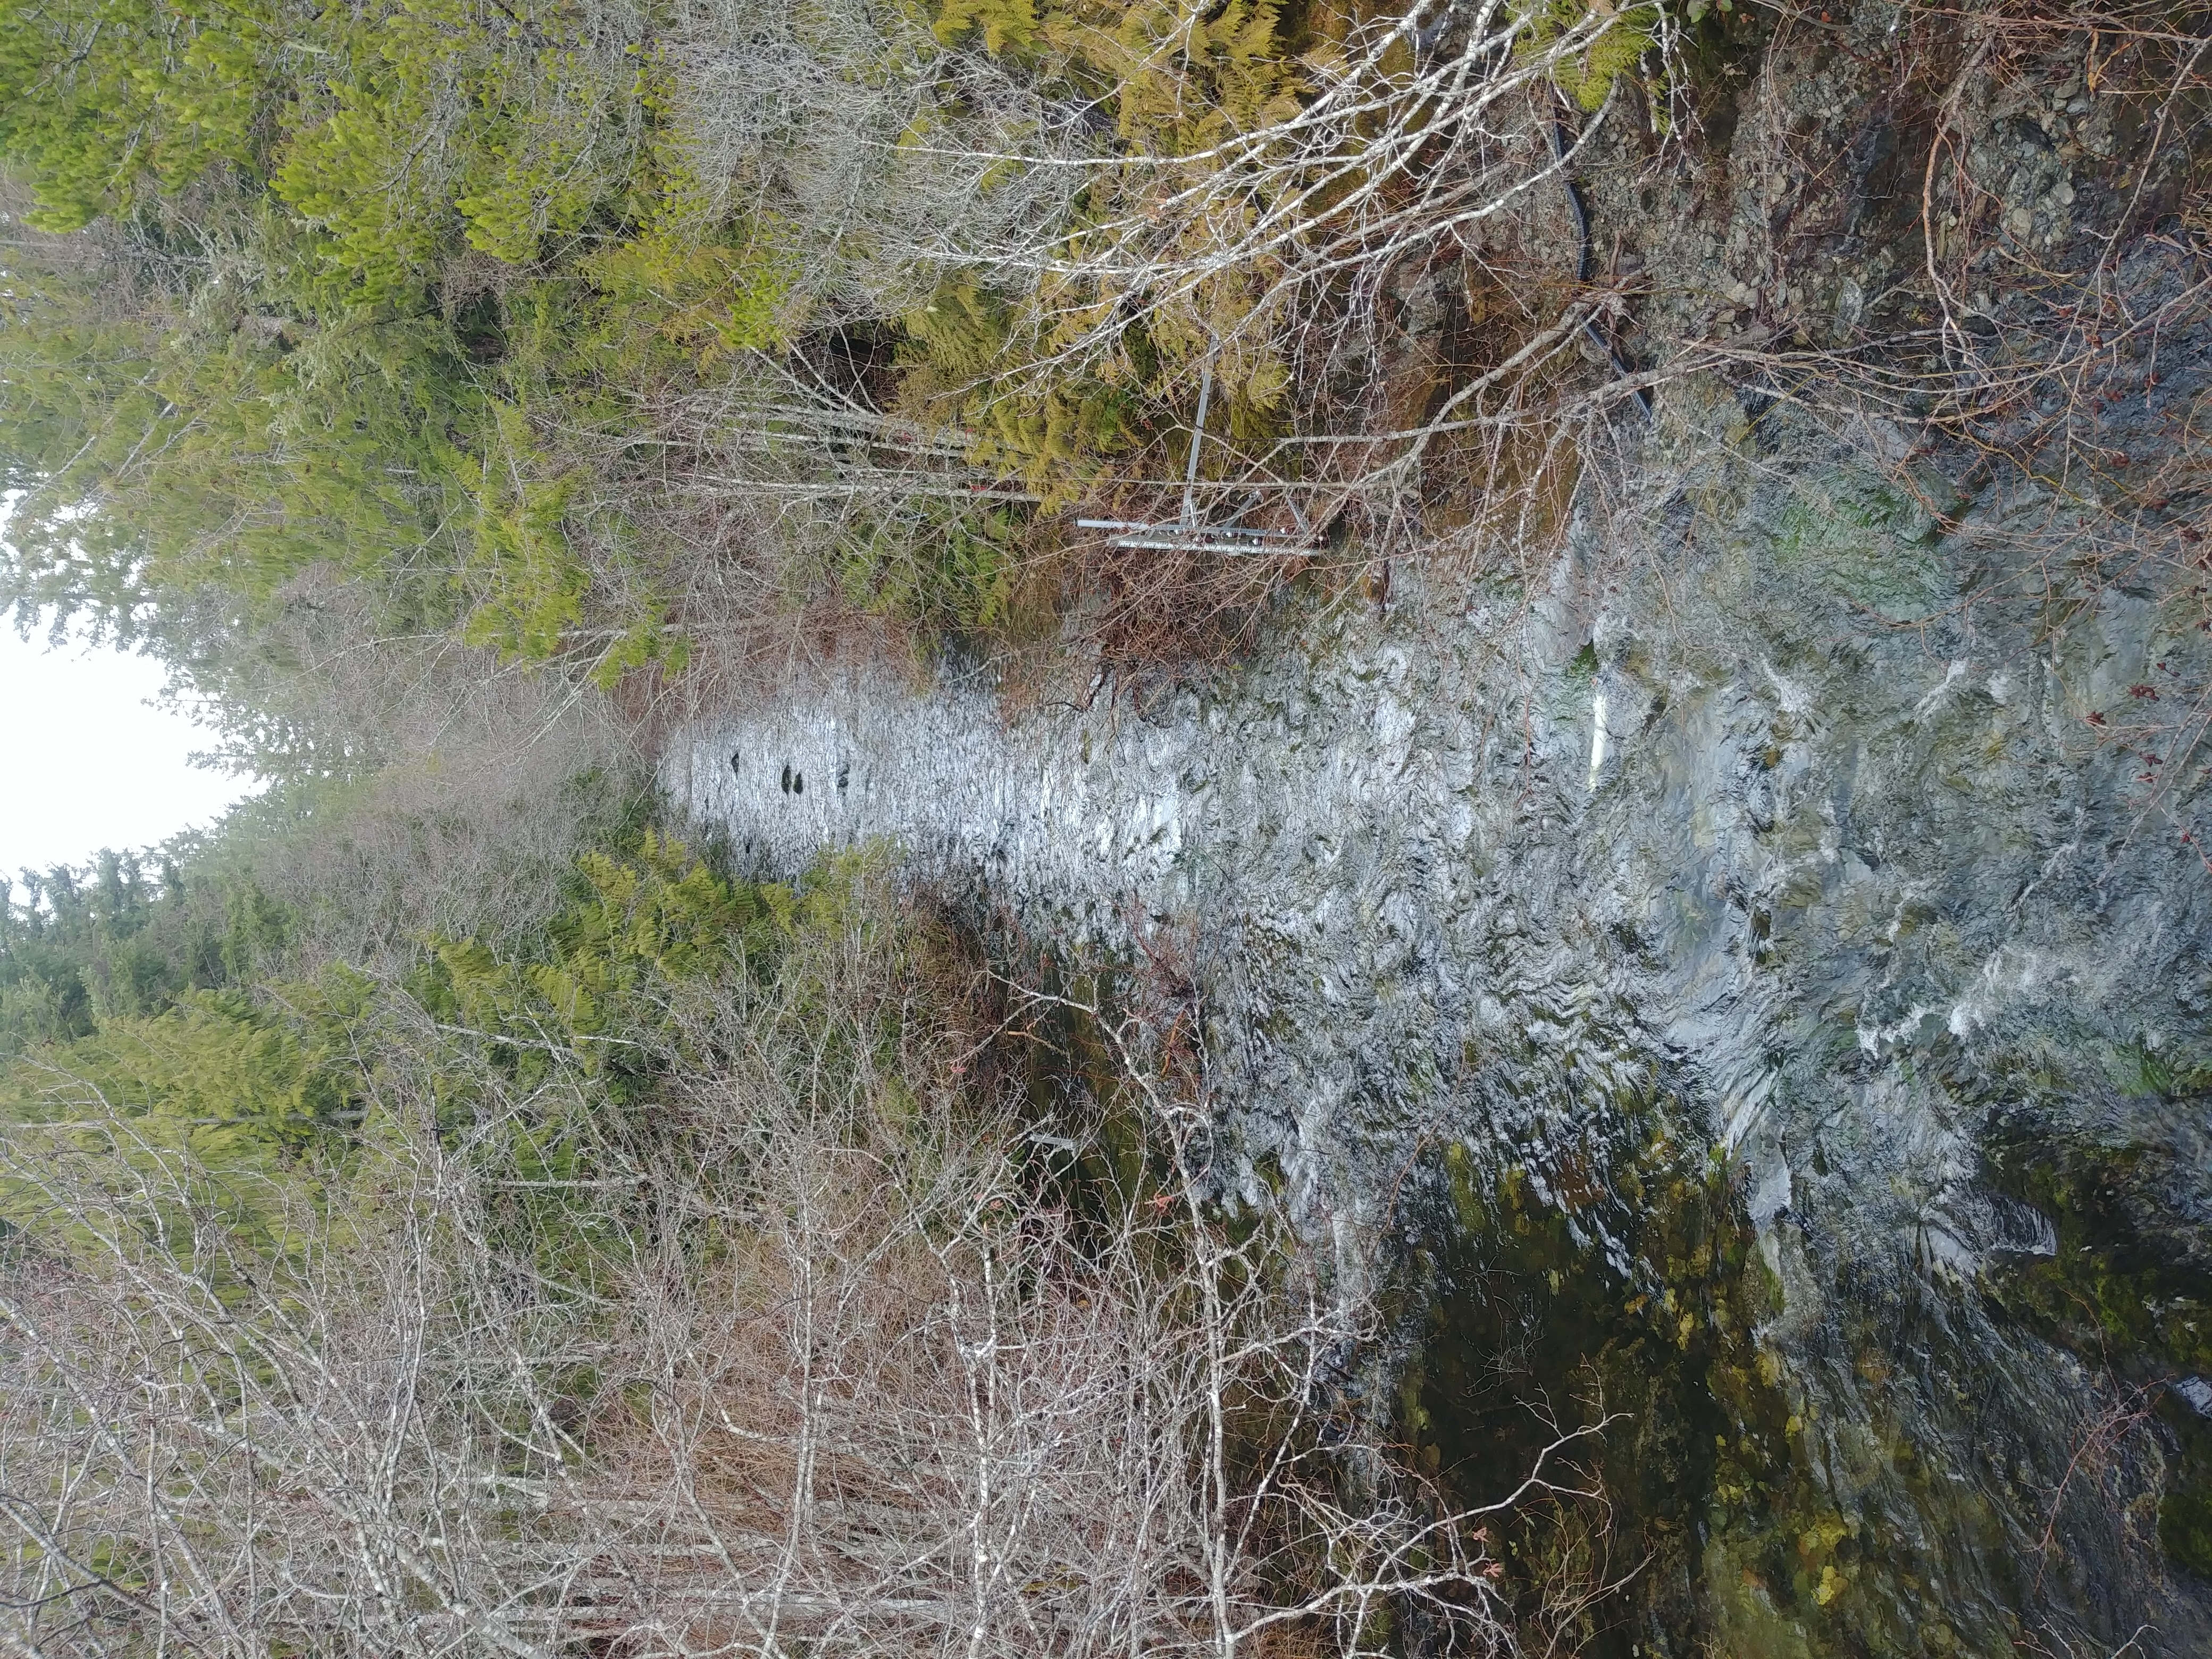
\includegraphics{images/Cragg_upstream_20190410.jpg}

\paragraph{5. West Leech}\label{west-leech}

Originating in the west of the Leech River watershed, West Leech River
is a 4th order mainstem river. The West Leech research site monitors a
drainage area of approximately 35 km\textsuperscript{2}. This reasearch
site has boulder and bedrock substrate, fairly straight channel with
relatively high width-to-depth ratio and pool-riffle morphology. The
West Leech site is approxiamtely 120m upstream of the confluence with
Leech mainstem (\textasciitilde{}1.5km downstream of the confluence of
Cragg Creek with Leech River).

\begin{figure}
\centering
\includegraphics{images/WestLeech_lowflow_20180828}
\caption{}
\end{figure}

\paragraph{6. Leech Tunnel}\label{leech-tunnel}

This research site is at the point of future diversion, the Leech
Tunnel. The Leech River is 5th order, and this research site has a
drainage area of approximately 99 km\textsuperscript{2}. The streambed
here is dominated by Schist bedrock and boulders. The bedrock in the
center of the channel is deeply incised, but overall the river is wider
than is is deep. The Tunnel site is approximately 1km downstream of the
West Leech confluence.

\begin{verbatim}
 ![](images/XXXXXXX.jpg){width=30%, style="float:left; padding:10px"}
\end{verbatim}

\section{Sampling Methods}\label{sampling-methods}

\subsection{Vertical racks for passive water sampling on the rising limb
of
hydrograph}\label{vertical-racks-for-passive-water-sampling-on-the-rising-limb-of-hydrograph}

\subsubsection{Theory}\label{theory}

\subsubsection{Design}\label{design}

\subsubsection{Benefits, challenges and
assumptions}\label{benefits-challenges-and-assumptions}

\subsubsection{Field protocol}\label{field-protocol}

\subsubsection{Method QA/QC: rising limb sampler quality assurance and
quality
control}\label{method-qaqc-rising-limb-sampler-quality-assurance-and-quality-control}

\paragraph{Assumption validation: rack samples are stable from
collection to retrieval and
analysis}\label{assumption-validation-rack-samples-are-stable-from-collection-to-retrieval-and-analysis}

\subparagraph{Temperatures (above and below water on
racks)}\label{temperatures-above-and-below-water-on-racks}

\subparagraph{Hold-time experiments}\label{hold-time-experiments}

\paragraph{Assumption validation: samples collected are discrete (no
subsequent
mixing)}\label{assumption-validation-samples-collected-are-discrete-no-subsequent-mixing}

\subparagraph{Rising limb sampler discretion
analysis}\label{rising-limb-sampler-discretion-analysis}

\subsection{Development of a passive water sampler design for the
falling limb of hydrograph (falling limb
sampler)}\label{development-of-a-passive-water-sampler-design-for-the-falling-limb-of-hydrograph-falling-limb-sampler}

\subsubsection{Theory}\label{theory-1}

\subsubsection{Design}\label{design-1}

\subsubsection{Benefits, challenges and
assumptions}\label{benefits-challenges-and-assumptions-1}

\subsubsection{Field protocol}\label{field-protocol-1}

\subsubsection{Method QA/QC: falling limb sampler quality assurance and
quality
control}\label{method-qaqc-falling-limb-sampler-quality-assurance-and-quality-control}

\paragraph{Assumption validation: samples collected are discrete (no
premature
infiltration)}\label{assumption-validation-samples-collected-are-discrete-no-premature-infiltration}

\subparagraph{Falling limb sampler discretion
analysis}\label{falling-limb-sampler-discretion-analysis}

\section{Analysis}\label{analysis}

\subsection{In the field: gauging
streamflow}\label{in-the-field-gauging-streamflow}

\subsubsection{Cross-sectional area and
velocity}\label{cross-sectional-area-and-velocity}

\paragraph{Weeks Outlet}\label{weeks-outlet-1}

\subsubsection{Manning's equation}\label{mannings-equation}

\paragraph{Leech Head}\label{leech-head-1}

\subsubsection{Salt dilution}\label{salt-dilution}

\paragraph{Chris Creek}\label{chris-creek-1}

\paragraph{Cragg Creek}\label{cragg-creek-1}

\paragraph{West Leech}\label{west-leech-1}

\subsection{In the laboratory: measuring water quality
parameters}\label{in-the-laboratory-measuring-water-quality-parameters}

\subsubsection{Quantitative analytical methods for dissolved organic
carbon}\label{quantitative-analytical-methods-for-dissolved-organic-carbon}

\paragraph{Direct via catalytic combution: non-purgeable organic carbon
(Shimadzu
TOC-V)}\label{direct-via-catalytic-combution-non-purgeable-organic-carbon-shimadzu-toc-v}

\paragraph{Proxy via spectrophotometry: optical absorbance (Scan
Spectrolyser)}\label{proxy-via-spectrophotometry-optical-absorbance-scan-spectrolyser}

\subsubsection{Qualitative analytical
methods}\label{qualitative-analytical-methods}

\paragraph{Molecular character of organic matter via fluorescence
excitation emission (Horiba
Aqualog)}\label{molecular-character-of-organic-matter-via-fluorescence-excitation-emission-horiba-aqualog}

\subsubsection{Ancillary data: contributions from
partners}\label{ancillary-data-contributions-from-partners}

\begin{itemize}
\tightlist
\item
  CRD FWx

  \begin{itemize}
  \tightlist
  \item
    Chris Creek weather station
  \item
    Martin's Gulch weather station
  \end{itemize}
\item
  CRD turbidity
\item
  CRD flow (Cragg, Judge, Rithet, Tunnel?)
\item
  CRD metals
\item
  forWater tretability \#\#\# Laboratory QA/QC: quality assurance and
  quality control \#\#\#\# Instrument calibration \#\#\#\# Calibration
  verification (cal vers)
\end{itemize}

\section{Results \& Discussion}\label{results-discussion}

\subsection{Spatial variability: DOC variability across the
watershed}\label{spatial-variability-doc-variability-across-the-watershed}

\subsubsection{Synoptic grab sampling at ten
locations}\label{synoptic-grab-sampling-at-ten-locations}

\subsubsection{Stormflow samples: compare and contrast six
sites}\label{stormflow-samples-compare-and-contrast-six-sites}

\subsection{Temporal variability: DOC variability over time and within
stormflow}\label{temporal-variability-doc-variability-over-time-and-within-stormflow}

\subsubsection{Seasonal patterns over sixteen months of
data}\label{seasonal-patterns-over-sixteen-months-of-data}

\subsubsection{Stormflow samples: variability within six
sites}\label{stormflow-samples-variability-within-six-sites}

\section{Conculsions}\label{conculsions}

\subsection{Characterizing the Leech Water Supply
Area}\label{characterizing-the-leech-water-supply-area}

\subsection{Understanding spatial and temporal variability in
hydrochemical
dynamics}\label{understanding-spatial-and-temporal-variability-in-hydrochemical-dynamics}

\section{Future Directions}\label{future-directions}

\begin{itemize}
\tightlist
\item
  How will source water with higher tannins (i.e Leech River water)
  affect the primary treatment process of UV disinfection (currently
  used for Sooke rerservoir water)?

  \begin{itemize}
  \tightlist
  \item
    What are the operational limits of TOC (or tannins) in source water
    with respect to UVT system performance?
  \end{itemize}
\item
  Can UVT photodegrade TOC molecules such that DBP-FP is reduced?
\item
  Can UVT be used as a primary treatment to reduce the requirements for
  chemical filtration and reduce the solid waste generated by
  coagaulants?
\end{itemize}

\section{References}\label{references}

\section{APPENDIX}\label{appendix}

\subsection{forWater: NSERC Strategic Network for forested drinking
water source protection
technologies}\label{forwater-nserc-strategic-network-for-forested-drinking-water-source-protection-technologies}

The forWater Network is a transdisciplinary cross-Canada applied
research collaboration focused on the connections between treated
drinking water quality and land-use impacts of forest management. The
majority of source drinking water originates in forested headwaters, but
the connection between upstream forest management and downstream
treatment remains poorly understood. Across Canada, forWater researchers
are studying water quality in watersheds under a variety of different
forest management strategies. Through collaborative analyses, forWater
is working to evaluate source water treatability metrics, downstream
propagation effects, and resource economic with the ultimate goal of
providing a framework for treatement demands as they relate to forest
management strategies.

\begin{figure}
\centering
\includegraphics[width=0.25000\textwidth]{images/SourceWater-forWater_smartart.jpg}
\caption{forWater NSERC Network for Forested Drinking Water Source
Protection Technologies}
\end{figure}

\begin{figure}
\centering
\includegraphics[width=0.50000\textwidth]{images/forWater_smartart.jpg}
\caption{forWater NSERC Network for Forested Drinking Water Source
Protection Technologies}
\end{figure}

\begin{figure}
\centering
\includegraphics[width=0.50000\textwidth]{images/forWater_themes.jpg}
\caption{forWater Research Themes}
\end{figure}

\hypertarget{refs}{}
\hypertarget{ref-CapitalRegionDistrict2017}{}
Capital Region District, Integrated Water Services. 2017. ``Regional
Water Supply 2017 Strategic Plan.'' Victoria, B.C.


\end{document}
